\section{Motivation and Related Work}

Most optimization schemes can be explained by choosing an approximation 
\(\hat{\Loss}\) for the \(\Loss\) function to be minimized, minimize that
approximation \(\hat{\Loss}\) instead and use the minimum as our next guess.
The approximations are typically simple, easy to minimize functions.

\begin{figure}
	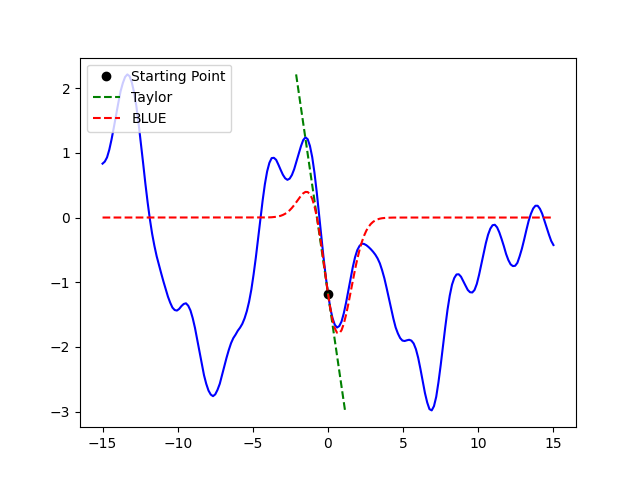
\includegraphics[scale=0.7]{graphics/BLUEvsTaylor3.png}
	\caption{
		A centered Gaussian Random Field with squared exponential covariance
		function is approximated by \(\param \mapsto \BLUE[\Loss(\param)\mid
		\Loss(0),\grad\Loss(0)]\). For comparison the first Taylor
		approximation in zero is also plotted. 
	}
\end{figure}

\begin{itemize}
	\item 
	The Newton-Raphson method is an immediate result of the second taylor approximation
	\begin{equation*}
		\hat{\Loss}_{N}(\param + \step)
		:= T^2_\param \Loss(\param + \step)
		= \Loss(\param)
		+ \langle \grad\Loss(\param), \step\rangle
		+ \tfrac12 \langle \grad^2\Loss(\param) \step, \step\rangle.
	\end{equation*}
	Optimizing \(\hat{\Loss}_{N}\) yields
	\begin{equation*}
		\step^*_{N} := -[\grad^2\Loss(\param)]^{-1}\grad\Loss(\param)
		= \argmin_\step \hat{\Loss}_{N}(\param + \step),
	\end{equation*}
	assuming the hessian \(\grad^2\Loss(\param)\) is strictly positive definite.

	\item
	Gradient Descent on the other hand is more conservative when it comes to its
	approximation. Using the fundamental theorem of calculus twice, to bound
	the approximation error of the first Taylor approximation implies 
	\begin{equation}\label{eq: T1 error}
		|\Loss(\param+\step) - T^1_\param \Loss(\param+\step)|
		= \left| \frac 12 \int_0^1 \step^T \grad^2\Loss(\param + \lambda \step)\step d\lambda\right|
		\le \tfrac{\ubound}2 \|\step\|^2,
	\end{equation}
	assuming \(\grad^2\Loss \preceq \ubound\identity\) in the sense that \(\ubound\identity
	- \grad^2\Loss(\param)\) is weakly positive definite for all \(\param\). Or
	equivalently: assuming all eigenvalues of \(\grad^2\Loss\) are smaller than
	\(\ubound\). From this we obtain
	\begin{equation*}
		\Loss(\param + \step) \le \hat{\Loss}_G(\param+\step)
		:= T^1_\param \Loss(\param+\step) + \tfrac{\ubound}2\|\step\|^2
	\end{equation*}
	with the approximation \(\hat{\Loss}_{G}\), we again find an analytical
	solution
	\begin{equation*}
		\step^*_{G} := - \frac1\ubound \grad\Loss(\param)
		= \argmin_\step \hat{\Loss}_{G}(\param + \step).
	\end{equation*}
\end{itemize}

The ``learning rate'' \(\frac1\ubound\) represents the answer to the question:
For how long can we trust the first taylor approximation? I.e. how fast does
the slope change and stop pointing downwards? And that rate of change of the
slope (gradient) is the Hessian which we assume is bounded by \(\ubound\).

Of course the curvature -- the rate the gradient changes -- is different from
function to function. That rate might not even be bounded, but even if it is,
we generally do not know this bound \(\ubound\). There are essentially two ways
to deal with this
\begin{enumerate}
	\item \textbf{Estimate and Bound}: We need the Hessian over the entire distance
	from \(\param\) to \(\param + \step\) to bound our approximation error in
	\eqref{eq: T1 error}, but maybe \(\grad^2\Loss(\param)\) is a good enough
	estimate? It might be, if the Hessian does not change too fast. So we need
	to bound the rate of change of the Hessian\footnote{
		``Cubic regularization'' is how \textcite[Section
		4.1]{nesterovLecturesConvexOptimization2018} constructs his second-order
		optimization scheme. But this scheme is not well known even though ``none
		of these [other] approaches seems to be useful in addressing the global
		behavior of second-order schemes'' \parencite[p.
		242]{nesterovLecturesConvexOptimization2018}. This is likely because cubic
		regularization is not analytically solvable. So it has very expensive
		steps.
	} to figure out for how long we can
	trust... déjà vu! We started out trying to figure out for how long we
	can trust the gradient. Now we are asking the same question about the
	Hessian. In other words: This approach only shifts the issue into the next
	derivative.

	For any Taylor polynomial \(\hat{\Loss}\) of \(n\)-th degree, we can always
	find a polynomial \(\Loss\) of \((n+1)\)-th degree with \(\hat{\Loss}\) as
	its \(n\)-th Taylor polynomial but with an arbitrarily high \(\Loss(\param +
	\step)\).

	\item \textbf{Guess and Try}: We could guess that the gradient does not
	change faster than rate \(\ubound\) and try the learning rate \(\frac1\ubound\).
	If we make progress, great, otherwise we double our guess of \(\ubound\),
	i.e. half the learning rate. Doing this every step is called backtracking. A
	check whether we have made a sufficient improvement is Armijo's rule. Using
	this rule, we can in fact optimize arbitrary \(C^1\) functions
	\parencite{truongBacktrackingGradientDescent2019}. In a stochastic gradient
	setting, we obviously do not know whether we made progress in one particular
	step. So backtracking becomes impossible. Therefore people tend to do an
	entire ``training run'' before they try out different ``hyperparameters'',
	i.e.  try out a different learning rate in the gradient descent case.
	\fxnote{Example: Sum of two different parabolas? Can't use Armijo's rule sequentially}
\end{enumerate}

Since the first approach eventually still leads to the second approach for some
higher derivative, we will have to guess eventually. The question is: What is
a good way to guess? If you start with a learning rate which ``\emph{usually}
works'', then you are already making a probabilistic statement: ``When drawing a
Loss function from a class of loss functions people are generally interested in,
a particular learning rate is \emph{likely} to work''.

So we want to assume that our loss function \(\Loss\) is the realization of a
random field.

\subsection{Bayesian Optimization}

\(\Loss\) being a random field is the setting assumed in Bayesian Optimization
\parencite[e.g.][]{frazierBayesianOptimization2018}. To find the minimum
of \(\Loss\) one could:

\begin{enumerate}
	\item Maximize the \emph{expected improvement} 
	\begin{equation}\label{eq: expected improvement}
		\EI(\param) := \E\big[
			[\hat{\Loss}_n^*- \Loss(\param)]^+
			\bigm|
			\Loss(\param_1),\dots, \Loss(\param_n)
		\big]
	\end{equation}
	over \(\param\), with
	\begin{equation*}
		\hat{\Loss}_n^* := \inf\{\Loss(\param_1),\dots, \Loss(\param_n)\}
		\quad \text{and} \quad
		[x]^+ := \max\{x, 0\}.
	\end{equation*}

	\item If we had to guess the minimum after \(n\) guesses, then we might
	choose
	\begin{equation*}
		\hat{\param}^*_n
		:= \argmin_{\param} \E[\Loss(\param)\mid \Loss(\param_1), \dots, \Loss(\param_n)].
	\end{equation*}
	in that case our expected improvement is what is called the \emph{knowledge gradient}
	\begin{equation*}
		\KG(\param_{n+1}) := \E[
			\Loss(\hat{\param}^*_n) - \Loss(\hat{\param}^*_{n+1})
			\mid \Loss(\param_1), \dots, \Loss(\param_n), \param_{n+1}
		],
	\end{equation*}
	we then pick our next evaluation by maximizing it.	
\end{enumerate}

A much more detailed comparison can be found in \cite{frazierBayesianOptimization2018},
but here is a rough explanation why the knowledge gradient might be better
(albeit even more difficult/expensive to compute than the expected improvement):
To maximize the expected improvement, the decision maker is forced to pick the
place they think will result in the smallest loss. In case of the knowledge
gradient on the other hand, the decision maker can pick a \(\param_{n+1}\) which
maximizes their \emph{information} about the loss \(\Loss\) instead, since they
are still allowed to pick a more conservative \(\hat{\param}^*_{n+1}\)
afterwards to measure the impact that evaluation had. The \emph{expected improvement}
optimizer is essentially too conservative in the exploration-exploitation trade-off. 

Bayesian Optimization requires distributional knowledge
about the loss \(\Loss\) which so far manifested in the assumption, that
\(\Loss\) is a Gaussian random field. And while the steps of Bayesian
Optimization are quite good, they are also quite expensive to choose. And this
expense scales poorly with the dimension.

So these methods are only used, when the input dimension of \(\Loss\) is small
and the cost of evaluating \(\Loss\) is extremely expensive, and therefore
justifies long/expensive deliberation where to evaluate next. How is it of
relevance for machine learning then? Well, it is used for the meta-optimization
problem of finding the right hyperparameters, where every evaluation of the loss
requires a complete retraining of the model.

We want to do something cheaper instead and use it to do optimization directly.

\subsection{Loss Surface Analysis}

In their seminal work \citetitle{dauphinIdentifyingAttackingSaddle2014}
\textcite{dauphinIdentifyingAttackingSaddle2014} suggest that we
should view the loss function \(\Loss\) as the realization of an isotropic,
centered Gaussian fandom field. Using this assumption they were able to use an
analysis of the distribution of critical points of such a random field
\parencite{brayStatisticsCriticalPoints2007}, to argue, that saddle points are
much more common in high dimension than local minima, and that the local minima
that do exist are overwhelmingly likely close to the global minimum. Intuitively
in high dimension the Hessian has many eigenvalues, all of which have to be
positive to result in a local minimum. This only happens when the loss is
close to the global minimum. They confirmed their predictions about critical
points on the MNIST dataset.

